\chapter{Analyse des besoins}

Le projet s'axe sur le besoin fonctionnel de base de l'interface graphique autour duquel gravitent des besoins non fonctionnels mais nécessaires au bon fonctionnement de l'application.

\section{Besoins}

Après une analyse des besoins du projet, nous avons défini deux sous catégories. D'un côté, les besoins graphiques, de l'autre, les besoins liés à la syntaxe des formules.

\subsection{Interface Graphique}

L'interface graphique doit être ergonomique et \textit{user-friendly}, le but est d'accompagner les étudiants dans l'apprentissage de la logique du premier ordre de la manière la plus agréable possible. Pour cela un certain nombre d'exigences en terme de GUI ont été mis en place:

\begin{itemize}
\item un jardin représenté par une grille de taille fixe;
\item des fleurs pouvant être disposées sur le jardin et ayant un visuel différent selon leurs espèces, tailles et couleurs;
\item un menu permettant de positionner de nouvelles fleurs à la souris et d’en changer les caractéristiques;
\item  un menu permettant d’écrire et vérifier des formules de la logique du premier ordre à l’aide d’un clavier virtuel et d’une liste de 5 variables et de 20 constantes;
\item  un menu permettant de sélectionner une variable ou une constante;
\item  un clavier visuel permettant de sélectionner les connecteurs de la logique (not, et, ou, pour tout, etc.);
\item  un menu permettant de sauvegarder et de charger des jardins et/ou des ensembles de formules.
\end{itemize}

Aperçu du rendu souhaité :

\begin{figure}[!h]
\begin{center}
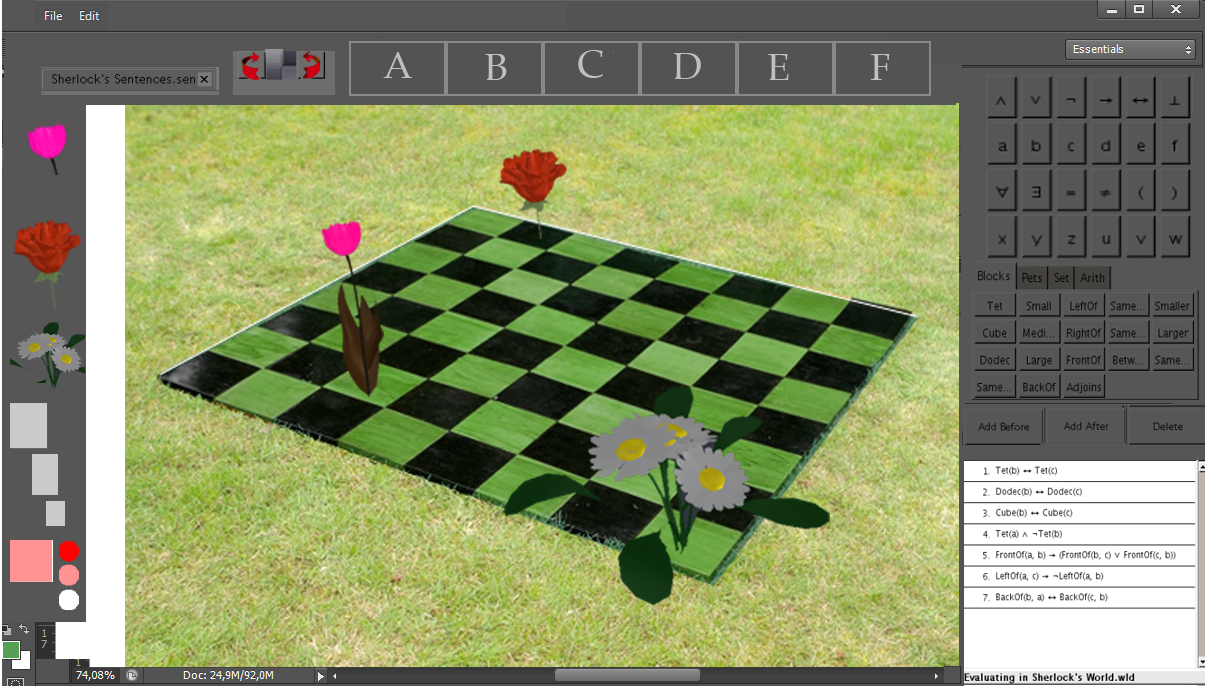
\includegraphics[height=10cm]{besoins/simulation.png}
\end{center}
\caption{Rendu attendu}
\end{figure}

\clearpage


\subsection{Analyse Syntaxique}

L'analyse syntaxique est un besoin lié directement au script fourni avec le sujet du projet. Si cette partie n'est pas parfaitement fonctionnelle, le script ne pourra donc pas fonctionner correctement et le projet ne pourra aboutir.\\
Idéalement, dans le cas d'une formule syntaxiquement fausse, l'analyseur pourra indiquer ou se trouve l'erreur dans la formule entrée par l'utilisateur. Cependant ce point n'est pas une nécessité, cette partie doit en priorité stopper le programme et notifier l'utilisateur du non respect de la syntaxe dans l'une de ses formules.\\

Il n'est utile d'aborder qu'un seul besoin non-fonctionnel: la communication entre deux langages différents, ce point étant technique nous préférons revenir dessus plus tard et seulement l'évoquer ici.
Il a cependant été pris en compte les contraintes de développement,  détaillées à la fin de cette partie.


\section{Développement}

Le développement est réparti en tâches parallélisées afin d'optimiser le temps de réalisation.

\subsection{Tâches}

Le développement s'axe sur trois grandes tâches, la communication inter langages, l'analyse syntaxique et la création de l'interface graphique. Le but étant de relier les trois blocs ensemble pour obtenir l'application finale.

%tableau à taille fixée sur certaines colonnes (param sur la ligne \begin{tabularx}, voir wiki pour plus d'info sur la syntaxe
\begin{figure}[!h]
\begin{center}
\begin{tabularx}{17cm}{|c|p{6cm}|X|}
  \hline
  Priorité & Nom & Raison\\
  \hline
  1 & Communication inter langages & Doit être vérifié en premier car sinon on ne pourra pas utiliser l'Analyseur Syntaxique \tabularnewline
  2 & Analyseur Syntaxique & On doit pouvoir entrer n'importe quel formule et être capable de détecter au plus vite la moindre erreur dans celle-ci \tabularnewline
  3 & Liaison Communication-Analyseur & Comme les principales fonctionnalités permettant de tester sont opérationnelles, nous pouvons passer à cette tâche. \tabularnewline
  4 & Création de l'interface graphique & Dernière fonctionnalité essentielle à mettre en place. \tabularnewline
  5 & Animation des fleurs & Non-essentiel, mais apporterait un plus au projet. \tabularnewline
  6 & Fonctionnalité de retour en arrière & Non-essentiel, mais apporterait un plus au projet. \tabularnewline
  \hline
\end{tabularx}
\end{center}
\caption{Tableau récapitulatif des tâches}
\end{figure}

\subsection{Organisation du code}

Dans le cas où l'analyseur syntaxique détecterait une erreur de formule, celui-ci ne retournera pas d'objets mais notifiera le bloc de communication de l'erreur. Ce dernier remontera donc le soucis au bloc GUI qui l'affichera à l'utilisateur.

\begin{figure}[!h]
\begin{center}
\includegraphics[height=10cm]{besoins/organisationProg.png}
\end{center}
\caption{organisation des blocs}
\end{figure}
